%!TEX root = ../paper.tex
\section{Video Classification in Caffe}
\label{sec:classification}

\subsection{Changes to Caffe-tmbo}

\begin{itemize}
	\item New sequence data layer
	\item Multi-layer script
	\item More?
\end{itemize}

\subsection{Spatial}
\label{subsec:spatial}

\begin{itemize}
	\item
		Different nets:
		\begin{itemize}
			\item Caffenet/CNN\_M (also tried, VGG 19, but too big)
			\item With weights/without weights
			\item Compare the nets with respect to memory, number of parameters, training time, performance
		\end{itemize}
	\item
		Experiments:
		\begin{itemize}
			\item Different dropouts
			\item Train from scratch vs train from weights
			\item On different splits?
			\item Fc6, Fc7, fc8
			\item Different base data sets (only 16, all data)
			\item Different flows?
			\item Occlusion tests
		\end{itemize}
	\item
		LSTM did not work out
\end{itemize}


\subsection{Flow}
\label{subsec:flow}


\subsection{Fusion}
\label{subsec:fusion}
As first approach we rebuild the fusion architecture presented by TODO.

We took the CNN nets for spatial and flow presented above and build a fusion architecture on top of them.
Both CNNs were cut off after the \textit{fc6}-layer having an output of 16 x 4096.\todo{Der eigentlich output von fc6 ist ja erstmal 1 x 4096}
The input to the CNNs were 16 frames per video.
So the output of the \textit{fc6}-layer of the spatial and flow net correspond to a prediction for each of those frames.
To fuse those predictions, the first step is to merge the 16 prediction of one video into one prediction for the whole video.
Therefore, we take the average prediction for both spatial and flow.
A fully-connected layer is then trained with those predictions before we concatenate the predictions of spatial and flow.
In the end two fully-connected layer are trained on the merged predictions.
The output is defined by an accuracy layer.
The whole architecture is shown in Figure~\ref{fig:fusion_architecture}\todo{improve figure}.
\begin{figure}[!htb]
	\centering
	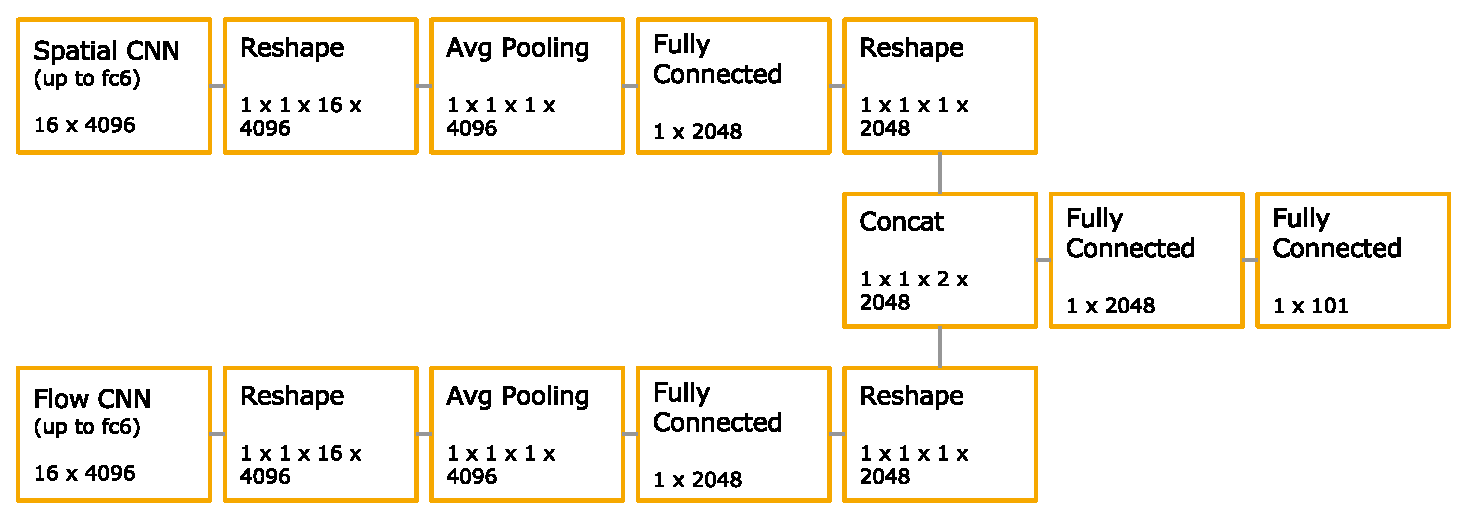
\includegraphics[scale=.7]{images/fusion_architecture.eps}
	\caption{Architecture of the fusion net: The predictions per frame of one video from the spatial and flow net are merged into one prediction per video each. Those predictions are then merged and trained via two fully connected layers.}
	\label{fig:fusion_architecture}
\end{figure}






